%!TEX root = ../thesis.tex
%Adding the above line, with the name of your base .tex file (in this case "thesis.tex") will allow you to compile the whole thesis even when working inside one of the chapter tex files
%: ----------------------- introduction file header -----------------------
\chapter{Thermal Energy Balance of Arcturus' Outflow}
\label{chap:7}

The chapter investigates the various heating and cooling processes that control the thermal structure of Arcturus' mass outflow region. We use the hybrid chromosphere and wind model derived in Chapter \ref{chap:6} as the basis to derive the magnitude of these processes as function of distance from the star. The analysis focuses on distances relatively close to the star (i.e., between $1.2$ and $10\,R_{\star}$) and includes the wind acceleration zone (i.e., between $\sim 1.2$ and $1.7\,R_{\star}$), a region where much of the energy that drives the wind is injected. The effect of adiabatic expansion cooling, line cooling from neutral and ionic species, and radiative recombination are investigated as wind coolants. The heating mechanisms investigated are the deposition of magnetic wave energy, ambipolar diffusion, and radiative heating. This work is a continuation of the initial findings of \cite{ogorman_2011}.

\pagebreak

\section{Motivation for a Thermal Energy Balance}\label{sec:7.1}
We have shown in Chapter \ref{chap:1} that for a monotonic ideal gas, the energy per unit mass, $e(r)$, is the sum of the kinetic and gravitational energies, and the enthalpy
\begin{equation}
\label{eq:7.1}
e(r)=\frac{v^2(r)}{2}-\frac{GM_{\star}}{r}+\frac{5\mathcal{R}T}{2\mu}.
\end{equation}
The lower boundary of a stellar outflow is the photosphere which is gravitationally bound to the star. This implies that the energy in Equation \ref{eq:7.1} must be negative at this point. If a star is to have an outflow, then the energy must become positive at large $r$ to escape the gravitational well (i.e., $v^2(r) \geq v_{\rm{esc}}^2(r)$). Therefore, energy must be added to the gas if the velocity is to reach (or exceed) the local escape velocity. The addition of this energy can be either in the form of heat input per unit mass, $q(r)$, or in the form of momentum input (i.e., an outward force per unit mass, $f(r)$; \cite{lamers_1999}). In other words, differentiating Equation \ref{eq:7.1} with respect to $r$ gives the change in energy per unit distance from the star, and this becomes
\begin{equation}
\label{eq:7.2}
\frac{d\,e(r)}{dr}=f(r)+\frac{dq(r)}{dr}
\end{equation}
which is just a form of the \textit{Bernoulli} equation. The unknown fundamental mechanisms responsible for driving the winds of cool evolved stars must therefore manifest themselves in either one or both of the quantities on the right hand side of Equation \ref{eq:7.2}. Therefore, studying the heating deposition, $q(r)$, taking place in Arcturus's outflow, is a valuable exercise and should provide insight into its wind driving mechanism(s).

Our multi-wavelength radio study of Arcturus allowed us to refine its existing atmospheric model. We found that our long wavelength VLA flux density measurements could be reproduced by the existing model if the almost isothermal outflow was replaced with an outflow that contained a large thermal gradient. This new hybrid model is graphically summarized in Figure \ref{fig6.9.3}. The goal in this chapter is to use this new model as a foundation to study the thermal energy balance in Arcturus's atmosphere. The simple idea behind this is that all the heating and cooling processes taking place in the outflow should combine to produce the derived thermal profile from Chapter \ref{chap:6}. Knowing the main mechanisms through which the plasma can cool thus allows us to examine the possible mechanisms which heat the plasma to the known temperature. Investigating the magnitude of the heating deposition of various mechanisms then tells us if such a mechanism can play a part in the mass-loss process.

\section{Thermal Model for a Spherically Symmetric Outflow}\label{sec:7.2}
In this section we derive an expression to describe how the temperature in a stellar outflow changes as a function of distance from the star. In doing so, we also present the notation that is used in subsequent sections to describe the magnitude of the heating and cooling taking place at certain regions in a stellar outflow. We assume all quantities vary radially (i.e, spherical symmetry) and that the mass-loss rate is constant (i.e., time independent). The continuity equation can then be written as
\begin{equation}
\label{eq:7.3}
v\frac{d\rho}{dr}=-\rho \left(\frac{dv}{dr}+\frac{2v}{r} \right)
\end{equation}
where $v$ and $\rho$ are the flow velocity and mass density at a distance $r$ from the star. The first law of thermodynamics tells us that the change in internal energy of a system is equal to the heat added to the system minus the work done by the system on its environment. For a reversible process in a closed system the work done is $PdV$, where $P$ and $V$ are the pressure and volume of the system. Writing the first law of thermodynamics in terms of rates per unit mass then gives
\begin{equation}
\frac{du}{dt}=\frac{dq}{dt}-\frac{P}{m}\frac{dV}{dt}
\end{equation}
where $u$ is the internal energy per unit mass and $q$ is the net heat gained per unit mass. The time dependence in the first and last terms can be switched to a radial dependence via $v=dr/dt$, and $m/\rho$ can be substituted for $V$ to get
\begin{equation}
v\frac{du}{dr}=-\frac{P}{\rho}\left(v\frac{d\rho}{dr} \right)+\frac{dq}{dt}.
\end{equation}
Substituting in Equation \ref{eq:7.3} and using $u=3nkT/2\rho$ and $P=nkT$ gives
\begin{equation}
v\left(\frac{3nk}{2\rho}\frac{dT}{dr}\right)=-\frac{nkT}{\rho}\left(\frac{dv}{dr} + \frac{2v}{r}\right) +\frac{dq}{dt}.
\end{equation}
If we define $\Gamma$ and $\Lambda$ as the heating and cooling rates per unit volume respectively, then we can rearrange this equation to get
\begin{equation}
\frac{dT}{dr}=-\frac{4T}{3r}-\frac{2T}{3v}\frac{dv}{dr}+\frac{2(\Gamma-\Lambda)}{3nkv}.
\end{equation}
The first two terms on the right account for adiabatic expansion cooling. The second term is important in the wind acceleration region but is zero once the wind has reached its terminal velocity. The third term accounts for all other heating and cooling processes. This equation is equivalent to Equation 8 in \cite{goldreich_1976} and can also be written in dimensionless form \citep{rodgers_1991} by multiplying across by $r/T$ as follows:
\begin{equation} 
\label{eq:7.8}
\frac{d(\mathrm{ln}\,T)}{d(\mathrm{ln}\,r)}=-\frac{4}{3}-\frac{2}{3}\frac{d(\mathrm{ln}\,v)}{d(\mathrm{ln}\,r)}+\displaystyle\sum_{i=1}\mathcal{H}_{i}-\displaystyle\sum_{j=1}\mathcal{L}_{j}
\end{equation} 
where 
\begin{equation}
\mathcal{H}_{i}=\frac{2r}{3nkvT}\Gamma_{i} 
\end{equation} 
and 
\begin{equation}
\label{eq:1.10}
\mathcal{L}_{j}=\frac{2r}{3nkvT}\Lambda_{j}
\end{equation} 
are the various heating and cooling rates per unit volume respectively, normalized to constant velocity adiabatic expansion cooling. Finally, this equation can be expressed in terms of the gas kinetic temperature's local power law slope, $\lambda$, 
\begin{equation} \label{eq:lambda}
\frac{d(\mathrm{ln}\,T)}{d(\mathrm{ln}\,r)}=-\lambda
\end{equation}
where 
\begin{equation}
\lambda =\lambda_{0}+\displaystyle\sum_{i=1}\lambda_{i}
\end{equation} 
which contains all of the wind heating and cooling processes, including that from adiabatic expansion cooling, $\lambda_{0}$. We note that positive and negative $\lambda$ values represent heating and cooling, respectively. This notation will be used throughout this chapter and allows the various heating and cooling process to be easily compared to the $4/3$ exponent, characteristic of a constant velocity outflow undergoing adiabatic expansion cooling.

\section{Cooling Processes}\label{sec:7.3}
The three ways in which the gas in Arcturus' partially ionized outflow can cool are through adiabatic expansion, radiative recombination, and collisional excitation of neutral and ionized atoms. We now assess the importance of each of these cooling processes between $\sim 1-10\,R_{\star}$. 

\subsection{Adiabatic Expansion Cooling}\label{sec:7.3.1}
Adiabatic expansion cooling is the thermodynamic process in which a fixed quantity of gas cools as it expands into a larger volume of gas. It is composed of a geometric term and a velocity gradient term; these being the first two terms on the right of Equation \ref{eq:7.8}. As shown in Figure \ref{fig:7.1}, the dominant term close to the photosphere is the velocity gradient term due to the rapid wind acceleration, while farther out where the wind reaches its terminal velocity, the geometric term becomes dominant. Adiabatic expansion cooling is a very efficient cooling mechanism in stellar outflows. To demonstrate this we take the atmosphere of Arcturus as an example and assume the absence of all other heating and cooling mechanisms. Considering only the adiabatic geometric cooling factor, the gas temperature would decrease to 1\,K by $1500\,R_{\star}$ which would lower the gas temperature to below the cosmic background temperature. 

\begin{figure}[!ht]
\centering 
         \includegraphics[trim=0pt 0pt 0pt 0pt,clip, width=8cm,height=12cm, angle=90]{/home/eamon/thesis/thesis_template/7/adiab.ps}
\caption[Various cooling mechanisms in Arcturus' wind]{The net cooling from adiabatic expansion, radiative recombination, and Lyman $\alpha$ cooling in Arcturus' outflow. For adiabatic expansion cooling, the dominant term close to the photosphere is the velocity gradient term from Equation \ref{eq:7.8}, due to the rapid wind acceleration, while further out where the wind reaches its terminal velocity, the geometric term becomes dominant. Radiative recombination is also an important cooling mechanism between $\sim 1-4\,R_{\star}$. The Lyman $\alpha$ cooling function is very sensitive to $T$ and is the dominant cooling process out to $2.8\,R_{\star}$.}
\label{fig:7.1}
\end{figure}

\subsection{Radiative Recombination Cooling}\label{sec:7.3.2}
Radiative recombination is the process by which an electron is captured by an ion into a bound state $n$ with the emission of a photon. The overwhelming abundance of H along with it having a similar cross section for capture to heavier ions, means that it is by far the most important species to consider for this cooling process. The radiative recombination cooling rate is 
\begin{equation}
\Lambda = n_{HII}n_e  \alpha ^{n}\left(\frac{3}{2}kT\right) \ \ \ \ \ \rm{erg\,s^{-1}\,cm^{-3}}
\end{equation}
where $3kT/2$ is the average thermal energy of a captured electron and $\alpha ^{n}$ is the hydrogen recombination rate coefficient summed over $n$ levels. The hydrogen recombination rate coefficient excluding captures to the $n=1$ level is given as 
\begin{equation}
\alpha _{B}= \frac{2.06\times 10^{-11}}{T^{1/2}}\phi _{2}(\beta) \ \ \ \ \ \rm{s^{-1}\,cm^{3}}.
\end{equation}
$\phi _{2}(\beta)$ is a function that varies with temperature and has been tabulated for various temperatures by \citep{spitzer_1978}. Recombination to the ground state is excluded because the process produces another ionizing
photon that can be easily absorbed again, producing the net effect that the recombination had not occurred. The radiative recombination cooling contribution can then be calculated using Equation \ref{eq:1.10}, and as shown in Figure \ref{fig:7.1}, its contribution is significant between $\sim 1-4\,R_{\star}$. 

\subsection{Lyman-alpha Cooling}\label{sec:7.3.3}
Collisions between electrons and gas atoms (or ions) causes energy to be exchanged between the thermal kinetic energy of the gas and the internal energy of the individual gas atoms (or ions). Collisional excitation cools the gas while collisional de-excitation heats the gas. At temperatures of a few thousand degrees, the excited levels in neutral hydrogen can become populated from electron collisions and thus can be a source of cooling. The analytical expression for the resulting net cooling rate per volume is
\begin{equation}
\label{eq:ly_alpha}
\Lambda _{\rm{eH}} = 7.3\times 10^{-19}n_{\rm{e}}n_{\rm{HI}}e^{-118,400/T(K)} \ \ \ \ \ \rm{erg\,s^{-1}\,cm^{-3}}
\end{equation}
\cite{spitzer_1978}. Most of the resulting radiation comes from the $n=2$ level (Lyman $\alpha$) and this is why the cooling rate is almost proportional to exp$(-E_{12}/kT)$, where $E_{12}/k=118319\,K$. Equation \ref{eq:ly_alpha} is a very sensitive function of the gas temperature and as can be seen from Figure \ref{fig:7.1}, is the dominant cooling process out to $2.8\,R_{\star}$. The sharp falloff in temperature in Arcturus' outflow post $2.3\,R_{\star}$ results in this mechanism changing from being a very efficient cooling process within $2.3\,R_{\star}$ to having a negligible effect by $\sim 3.1\,R_{\star}$.

\subsection{Other Line Coolants}\label{sec:7.3.4}
Due to its large abundance, hydrogen is expected to be the most efficient line cooling mechanism in the inner atmosphere of Arcturus. Nevertheless, it is also worth investigating the effects of line cooling from heavier elements which may become important at lower temperatures further out in the atmosphere, where line cooling from H has almost ceased. Line cooling from these heavy elements is due mainly to electron impact excitation of electronic levels of the neutral and ionized species at high temperatures, while at lower temperatures (i.e. farther out in the CSE) line cooling is mainly due to the electron impact excitation of fine structure levels of the neutral and ionized constituents \citep{dalgarno_1972}. Table \ref{tab:7.1} lists the most relevant heavy elements for this study based on abundance and suitable line transitions. All heavy elements with an ionization potential (IP) lower than O were assumed fully ionized,  while the ionization balance of O was based on the \textit{IUE} line profile analysis of \cite{judge_1986}.

\begin{table}[!ht]
\begin{center}
\caption[Elemental Abundance in Arcturus's Outflow]{Elemental Abundance in Arcturus's Outflow.}
\begin{tabular}{cccc}
\hline
\hline
\rule{0pt}{2.5ex} Element & Abundance & IP (eV) & Reference \\
\hline
\rule{-2.5pt}{2.5ex}	O &  $4.7\times 10^{-4}$ & 13.6 & \cite{ramirez_2011}\\
					C &  $2.1\times 10^{-4}$ & 11.3 & \cite{ramirez_2011}\\
					N$^{1}$ &  $6.7\times 10^{-5}$& 14.5 & \cite{asplund_2009}\\
					Mg & $3.0\times 10^{-5}$ & 7.6 & \cite{ramirez_2011}\\
					Si & $2.0\times 10^{-5}$ & 8.2 & \cite{ramirez_2011}\\
					Fe & $1.0\times 10^{-5}$ & 7.9 & \cite{decin_2003}\\
\hline
\end{tabular}
\label{tab:7.1}
\begin{minipage}{12.5cm}
\rule{-2.5pt}{2.5ex}{\footnotesize $^{1}$\,Assumed solar abundance.}
\end{minipage}
\end{center}
\end{table}

The line cooling rate per unit volume due to the transition $ul$ in a medium where the optical depth is not negligible is 
\begin{equation}\label{eq:7.16}
\Lambda _{\rm{line}} =\sum_{u\rightarrow l} n_{u}A_{ul}E_{ul}\rho (\tau) \ \ \ \ \ \rm{erg}\,\rm{s^{-1}\,cm^{-3}}
\end{equation}
where $n_{u}$ is the population of the upper level, $A_{ul}$ is the spontaneous emission coefficient of the transition, and $E_{ul}$ is the energy of the radiated photon. Here, the sum is over all possible upper to lower transitions and $\rho (\tau)$ is the probability the photon will escape the gas without being reabsorbed. This function lowers the line cooling rate and can be written as 
\begin{equation}
\rho (\tau) = \frac{1-\mathrm{exp}(-3\tau /2)}{3\tau /2}\,.
\end{equation}
This expression reaches the correct solution in the low and high optical depth limits. It is used in the work of \cite{rodgers_1991} and is an approximation of \cite{castor_1970}'s escape probability when the logarithmic velocity gradient is zero.  The level populations in Equation \ref{eq:7.16} were found by solving the rate equations, which for a two level atom can be written as,
\begin{equation}
\frac{n_u}{n_l}=\frac{g_u}{g_l}\mathrm{exp} \left( \frac{-E_{21}}{kT}\right)\left( 1+\frac{n_{\mathrm{cr}}}{n} \right)^{-1}.
\end{equation}
Here $g_{u}$ and $g_{l}$ are the degeneracy (the number of states with the same energy) of the levels and $n$ is the number of collisional partners in the gas. The critical density, $n_{\rm{cr}}$, is the ratio of the radiative and collisional de-excitation rates
\begin{equation}
n_{\rm{cr}}=\frac{A_{ul}\rho _{ul}}{C_{ul}}
\end{equation}
and determines whether the gas is effectively thin at that point in the outflow.

\begin{figure}[!t]
\centering 
         \includegraphics[trim=0pt 0pt 0pt 0pt,clip, width=7cm,height=12cm, angle=90]{/home/eamon/thesis/thesis_template/7/tot_cooling.ps}
\caption[Summation of all cooling mechanisms]{Summation of all the cooling mechanisms normalized to constant adiabatic cooling taking place in Arcturus' outflow. The cooling taking place within the first $3\,R_{\star}$ is mainly due to Lyman Alpha, emission line while the cooling further out is from gas expansion, with a small contribution from radiative recombination.}
\label{fig:7.2}
\end{figure}

\begin{table}[!ht]
\begin{center}
\caption[Properties of the Strongest Line Coolants]{Properties of Strongest Line Coolants.}
\begin{tabular}{ccccc}
\hline
\hline
\rule{0pt}{2.5ex} Species & Transition & E$_{ul}$ (K) & $\lambda$ (\AA) & A$_{ul}$ (s$^{-1}$) \\
\hline
\rule{-2.5pt}{2.5ex}	\ion{C}{ii} &  ${}^{4}P \rightarrow {}^{2}P$ & $6.2\times 10^4$ & 2326& 3.6\\
						\ion{O}{i} &  ${}^{1}D \rightarrow {}^{3}P$ & $2.3\times 10^4$ & 6300&$6.7\times 10^{-3}$\\
						\ion{Mg}{ii} &  ${}^{2}S \rightarrow {}^{2}P$ & $5.1\times 10^4$ & 2796 & $2.6\times 10^8$\\

\hline
\end{tabular}
\label{tab:7.2}
\begin{minipage}{19.5cm}
{\footnotesize \rule{0pt}{2.5ex}\hspace{2.3cm} Note: Data taken from \cite{hollenbach_1989}.}
\end{minipage}
\end{center}
\end{table}


The line cooling from these heavy elements was found to be only significant within $1.5\,R_{\star}$; the most efficient of which being the \ion{C}{ii}\,$^{4}P \rightarrow {}^{2}P$  spin-forbidden permitted dipole multiplet (2326\,\AA). The properties of this feature, along with the next two strongest line coolants are shown in Table \ref{tab:7.2}. As the density decreases, so too do the number of collisions, and so when atoms/ions radiate they are less likely to be re-excited. Therefore line cooling from these heavy elements is only important at high densities, i.e., close to the star. In Figure \ref{fig:7.2} we plot the sum of all the cooling mechanisms taking place in Arcturus' outflow. The cooling taking place within the first $3\,R_{\star}$ is mainly due to Lyman Alpha emission line while the cooling further out is mainly due to gas expansion, with a small contribution from radiative recombination. 

\section{Heating Mechanisms}\label{sec:7.4}
In the following sections we investigate various possible heating mechanisms taking place in Arcturus's outflow and the  overall efficiency of these mechanisms at various distances from the star. 

\subsection{Photoionization Heating}\label{sec:7.4.1}
The UV radiation field of Arcturus can photoionize atoms producing energetic electrons which heat the atmosphere. The energy released per second per unit volume due to the photoionization of an atom $X$ can be written as
\begin{equation}\label{eq:7.20}
\Gamma (X) = n(X)\int ^{\lambda _{th}}_{\lambda _{min}}\frac{4\pi J_{\lambda}}{E _{\lambda}}\sigma _{X}(\lambda)(E_{\lambda} - E_{\lambda _{th}})d\lambda .
\end{equation}
Here, $E_{\lambda} - E_{\lambda _{th}}$ is the energy added to the gas by one ionization, i.e., the energy of the incident photon minus the threshold energy for ionization, which is specific to each element. $J_{\lambda}$ is the 
mean intensity of radiation at a point and so $4\pi J_{\lambda}/E _{\lambda}$ is the number of incident photons per unit area per unit time per unit wavelength interval. $\sigma _{X}(\lambda)$ is the ionization cross section for an atom $X$ by photons with an energy $E_{\lambda}$ below a threshold wavelength, $\lambda _{th}$, and is a function of wavelength.

\begin{figure}[!ht]
\centering 
         \includegraphics[trim=0pt 0pt 0pt 0pt,clip, width=8.5cm,height=13cm, angle=90]{/home/eamon/thesis/thesis_template/7/cross_secs.ps}
\caption[Photoionization cross section values]{The photoionization cross section values for atoms with IPs less than 13.6\,eV which were used in this study. The photoionization of H from the $n=2$ level was also considered and its cross section is also shown. The Balmer continuum is the ionization threshold for H\,(n=2) is 3646\,\AA .}
\label{fig:7.3}
\end{figure}

To calculate the mean intensity, the incident flux must be known. The flux at the stellar surface, $F_{\star}$, is related to the flux observed at Earth, $F_{\oplus}$, by
\begin{equation}
F_{\star}= \left(\frac{d}{R_{\star}}\right)^2F_{\oplus}=\left(\frac{2}{\phi}\right)^2F_{\oplus}
\end{equation}
where $d$ is the distance and $\phi$ is the angular diameter. The mean intensity at a point in the atmosphere is then
\begin{equation}
J(r)=W(r)I_{\star} =\frac{W}{\pi}\left(\frac{2}{\phi}\right)^2F_{\oplus}
\end{equation}
where $I_{\star}$ is the specific intensity and we have assumed the relationship, $F_{\star}=\pi I_{\star}$. $W(r)$ is the radiation dilution factor and is given by
\begin{equation}
W(r)=\frac{1}{2}\left(1 - \sqrt{1-\left(\frac{R_{\star}}{r}\right)^2} \right).
\end{equation}
The incident flux measurements (i.e., $F_{\oplus}$) which vary as a function of wavelength were obtained from the online StarCAT catalog \citep{ayres_2010}. Any missing data were interpolated or extrapolated upon to provide a continuous $J(r)$ between 912\,\AA and 3646\,\AA\,\,[i.e., the ionization threshold for the H\,($n=2$) level]. The photoionization cross section values for atoms with IPs less than 13.6\,eV along with the values for the H\,($n=2$) level were taken from \cite{mathisen_1984} and are shown as a function of wavelength in Figure \ref{fig:7.3}. 

The net heating due to photoionization was then found by using Equation \ref{eq:7.20} for each of these species resulting in significant heating inside $\sim 1.4\,R_{\star}$ as shown in Figure \ref{fig:7.5}. However, by $\sim 2\,R_{\star}$ its heating ability is about one order of magnitude weaker than adiabatic cooling at the same distance and so photionization heating is not an efficient mechanism in heating Arcturus' outflow.

\subsection{Ambipolar Diffusion Heating}\label{sec:7.4.2}
If a magnetic field remains frozen to the electrons and ions in a plasma, the charged plasma and field can drift through the gas of neutral atoms. The collisions, chiefly between positive ions and neutral hydrogen atoms \citep{spitzer_1978}, result in an exchange of momentum between the magnetic field and the neutral gas which results in a net heating. The recent possible detection of a weak ($B < 1\,G$) mean longitudinal magnetic field for Arcturus \citep{sennhauser_2011} suggests that ambipolar diffusion heating should be considered as a possible heating mechanism.  We use the expression given by \cite{shang_2002} to define the volumetric rate of ambipolar  diffusion 
\begin{equation}\label{eq:1.24}
\Gamma = \frac{\rho _{n}|\mathbf{f}_{L}|^2}{\gamma \rho _{i}(\rho _{n}+\rho _{i})^2}.
\end{equation}
Here, $\rho _{n}$ and $\rho _{i}$ are the mass densities of the neutral and ionic species, respectively, $\gamma$ is the ion-neutral momentum transfer coefficient (in units cm$^3$\,s$^{-1}$\,g$^{-1}$), and $\textbf{f}_{L}$ is the volumetric Lorentz force
\begin{equation}
\textbf{f}_{L}=\frac{1}{4\pi}(\grad \times \textbf{B})\times \textbf{B}
\end{equation}
where \textbf{B} is the magnetic field vector. In order to calculate the ambipolar diffusion heating, we need to find a value for $\gamma$, which depends on the collisional coefficient rates, cross sections, slip speed, and gas composition. The $\gamma$ coefficient can be transformed into a quartic equation by eliminating a term known as the slip velocity, $w$ ($w\equiv v_{i}-v_{n}$). The derivation of \ref{eq:1.24} assumes that the difference in acceleration in the neutrals and ions can be ignored. The radial Lorentz force is found from the equation of motion:
\begin{equation}
\rho _{n}v_{n}\frac{dv_{n}}{dr}+\rho _{i}v_{i}\frac{dv_{i}}{dr}=-\frac{GM_{\star}}{r^2}(\rho _{n} + \rho _{i})+f_{L}.
\end{equation}
This then allows the $\gamma$ coefficient and thus the volumetric heating to be calculated. The effect of radial ambipolar diffusion heating was found to be about three orders of magnitude less than adiabatic constant velocity expansion cooling and is therefore a negligible heating mechanism. This is due to the relatively high ionization balance in Arcturus' outflow.

\subsection{Turbulent Heating}\label{sec:7.4.3}
The dissipation of turbulent fluctuations can make a significant contribution to the thermodynamic heating of a plasma, and has regularly been studied as a heating source of the solar corona and driving solar wind acceleration \citep[e.g.,][]{lehe_2009, cranmer_2007}. It has also been studied as a source of energy and momentum for accelerating cool evolved stellar winds \citep[e.g.,][]{falceta_2006, hartmann_1980}. These studies have focused on the dissipation of turbulent fluctuations from Magnetohydrodynamic (MHD) waves and we likewise make the same assumption. However, our simple phenomenological description of turbulent heating can also be explained by the dissipation of acoustic waves in an unmagnetized medium \citep[e.g.,][]{lighthill_1952,stein_1967}.

\begin{figure}[!ht]
\centering 
         \includegraphics[trim=0pt 170pt 0pt 150pt,clip, scale=0.5]{/home/eamon/thesis/thesis_template/7/flux_tube.ps}
\caption[Example of diverging flux tubes]{Example of diverging flux tubes in the atmosphere of a cool evolved star. The filling factor, $f$, of the open magnetic flux tubes grows from $f_{\star} \ll 1$ at the photosphere to an asymptotic value of $f_{\infty} \rightarrow 1$ at large distances. Alfv\'en waves then propagate up these flux tubes and are partially reflected, resulting in an interaction causing turbulence which dissipates into heating. Image adopted from \cite{cranmer_2011}.}
\label{fig:7.4}
\end{figure}

The idea of MHD turbulent heating of Arcturus' atmosphere is based on what is known to happen in the solar atmosphere. For the Sun, most of the photospheric magnetic field is located in small flux tubes (of diameter $\sim 100$\,km) concentrated in the intergranular downflow lanes with field strengths of $\sim 1400$\,G \citep{berger_2001}. These flux tubes, whose geometries are shown in Figure \ref{fig:7.4}, have relatively small photospheric filling factors of $f_{\star} \sim 0.1-1\, \%$ and so the total magnetic flux density is much lower when spatially averaged over the entire solar disk and is in the order of $f_{\star}B_{\star}=1-10$\,G \citep{schrijver_1989}. The same structures may be present in the atmosphere of Arcturus, which possibly has of a weak ($B < 1\,G$) mean longitudinal magnetic field \citep{sennhauser_2011}. Alfv\'en waves then propagate up these flux tubes and are partially reflected by radial gradients in the density and magnetic field strength. The counter-propagating wave packets then interact with one another along these flux tubes, developing into strong MHD turbulence \citep{iroshnikov_1964}. The energy flux in the cascade from large to small eddies terminates in dissipation and heating \citep[e.g.,][]{matthaeus_1999, cranmer_2005}.

In this study, we adopt the following phenomenological form for the MHD turbulent heating rate per unit volume,
\begin{equation}
\Gamma_{turb} =\frac{1}{2}\frac{\rho U^{2}}{L/U}\ \ \ \rm{erg \ s^{-1} \ cm^{-3}}
\end{equation} 
where $U$ is the characteristic velocity and $L$ is the characteristic length scale. For solar studies, the characteristic length scale at the photosphere would be the size of the granular cells that are responsible for perturbing the flux tubes (i.e., $100-1000$\,km), which are similar in size to the solar photospheric density scale height (i.e, $H_{\odot} \sim 270$\,km). Unlike the Sun, we cannot determine $L$ via observations and choose $L$ to be the local density scale height:
\begin{equation}
L = \rho \left(\dfrac{d\rho}{dr} \right)^{-1}.
\end{equation}
The characteristic velocity is taken to be the local hydrogen sound speed, i.e., 
\begin{equation}
U=\sqrt{\frac{5}{3}\dfrac{P}{\rho}}=12.85\times 10^{5}\sqrt{\frac{T_{e}}{10^4}}\ \ \ \ \rm{cm}\,\rm{s}^{-1}.
\end{equation}
Observations of optically thin chromospheric lines show that the turbulent velocity is similar to the local sound speed and we make the assumption that this remains true throughout the outflow. 

This simple description of turbulent heating assumes an ideal \cite{kolmogorov_1941} hydrodynamic cascade but such simple descriptions have already successfully reproduced many properties of coronal heating for the Sun \citep{cranmer_2012}. The dissipation of turbulent fluctuations in Arcturus' wind make a significant heating contribution out to many stellar radii, as can be seen in Figure \ref{fig:7.5}. It can be shown that 
\begin{equation}
\lambda_{turb} \propto \frac{\sqrt{T_e}}{v}\frac{d(\mathrm{ln}\,\rho)}{d(\mathrm{ln}\,r)}
\end{equation} 
and so when the wind has reached its terminal velocity, the turbulent heating varies as $\lambda_{turb} \propto \sqrt{T_e}$.

\begin{figure}[!ht]
\centering 
         \includegraphics[trim=0pt 0pt 0pt 0pt,clip, scale=0.5,angle=90]{/home/eamon/thesis/thesis_template/7/tot_heating.ps}
\caption[Main heating mechanisms in Arcturus' wind]{The main heating mechanism in Arcturus' wind is from the dissipation of turbulence. Photoionization of H also contributes to heating close to the star, while the heating from ambipolar diffusion is found to be negligible.}
\label{fig:7.5}
\end{figure}

\section{Thermal Energy Balance}\label{sec:7.5}
We now consider the balance of heating and cooling for the reasons discussed at the end of Sections \ref{sec:7.1}.
We first find the gas kinetic temperature local power law slope, $\lambda$, for the new atmospheric model of Arcturus, which we developed in Chapter \ref{chap:6}. To do so, we substitute the temperature profile into Equation \ref{eq:lambda}. As the flow is isothermal between $1.2$ and $2.3\,R_{\star}$, the power law slope is zero as shown in Figure \ref{fig:7.6}. Beyond $2.3\,R_{\star}$, this model contains a temperature power-law slope of $T_e \propto r^{-1.65}$, and therefore $\lambda = -1.65$. For clarity, we have excluded the data within $1.2\,R_{\star}$ throughout this section as the density and temperature gradients within this region are very large, and can make the calculated $\lambda$ many orders of magnitude greater than those beyond $1.2\,R_{\star}$. The majority of the wind acceleration occurs beyond $1.2\,R_{\star}$ so the velocity gradient is still taken into account in our analysis.

\begin{figure}[!ht]
\centering 
         \includegraphics[trim=0pt 20pt 0pt 40pt,clip, scale=0.6,angle=90]{/home/eamon/thesis/thesis_template/7/therm_bal.ps}
\caption[Net thermal balance]{The gas kinetic temperature local power law slopes used for calculating the thermal energy balance. The green solid line is the power law slope of the new atmospheric model for Arcturus described in Chapter \ref{chap:6}. The blue dashed line is the net cooling as a result of combining all of the cooling and heating processes described in Sections \ref{sec:7.3} and \ref{sec:7.4}. The red dot-dashed line is the required additional heating/cooling to reproduce the thermal structure of our model atmosphere. A significant additional energy input is required within $3\,R_{\star}$ to reproduce our model atmosphere, while some additional cooling is required beyond $3\,R_{\star}$. }
\label{fig:7.6}
\end{figure}

In theory, if we were able to precisely account for all of the heating and cooling processes taking place in Arcturus' atmosphere, then a summation of their power law slopes would reproduce the power law slope of the model atmosphere (assuming the model atmosphere to be an exact representation of the actual atmosphere). The dashed blue line in Figure \ref{fig:7.6} represents a summation of all the heating and cooling processes discussed in Sections  \ref{sec:7.3} and \ref{sec:7.4}. The result of this is a considerable net cooling at all distances from the star. Within $\sim 3\,R_{\star}$, this net cooling far exceeds that predicted by the atmospheric model. This implies that one or more additional energy inputs must be acting on the inner region of of the outflow, which have not been accounted for in Section \ref{sec:7.4}. The magnitude of this required additional heating within $\sim 3\,R_{\star}$ is also shown in Figure \ref{fig:7.6} and is represented by the dot-dashed red line. Beyond, $\sim 3\,R_{\star}$ the temperature power law slope of the model atmosphere is less than the slope of the calculated net cooling. This is because the model atmosphere of Arcturus is cooling super-adiabatically beyond $2.3\,R_{\star}$ where $\lambda = -1.65$, while we have found that the only significant cooling process beyond $\sim 3\,R_{\star}$ is adiabatic expansion where $\lambda = -1.33$. 

\section{Discussion}\label{sec:7.6}
In Section \ref{sec:7.3} we found that the effect of Ly\,$\alpha$ line cooling becomes small beyond $\sim 3\,R_{\star}$ and at greater distances we found that the only efficient cooling mechanism is adiabatic expansion. Since the velocity gradient is zero at these greater distances, the temperature local power law slope is $\lambda = -1.33$. The fact that we have not found any other efficient cooling mechanism beyond $\sim 3\,R_{\star}$ does hint that the temperature power-law coefficient of $-1.65$, in the new atmospheric model for Arcturus, may be too severe. The fact that we assumed a constant ionization fraction when investigating the radio spectral indices in Chapter \ref{chap:6} (i.e., the ionization balance was assumed to be \textit{frozen-in}) may be a reason for this. Allowing the ionization balance to vary would have produced a smaller temperature power-law coefficient, but this approach would have given too many free parameters and no unique wind solution would have been attainable via our analytical approach. 

The value of the red dot-dashed line in Figure \ref{fig:7.6} would be zero at all radii if our model atmosphere was a complete description of the true value and if we had accounted for all of the heating and cooling processes. It is clear from this figure that the best results (i.e., closest values to zero) are found at distances beyond  $3\,R_{\star}$ where adiabatic expansion cooling produces a power law slope of $\lambda =-1.33$ which is reasonably close to the model value of $\lambda =-1.65$. However, within $\sim 3\,R_{\star}$, it is very clear that some major additional heating source is required to maintain the temperature profile of our model atmosphere. A more rigorous treatment (i.e., a non-phenomenological description) of heating due to the turbulent dissipation of Alfv\'en waves may be one possible route for further investigation, although one would wonder how the different descriptions of the same process could produce such vastly different results. 